

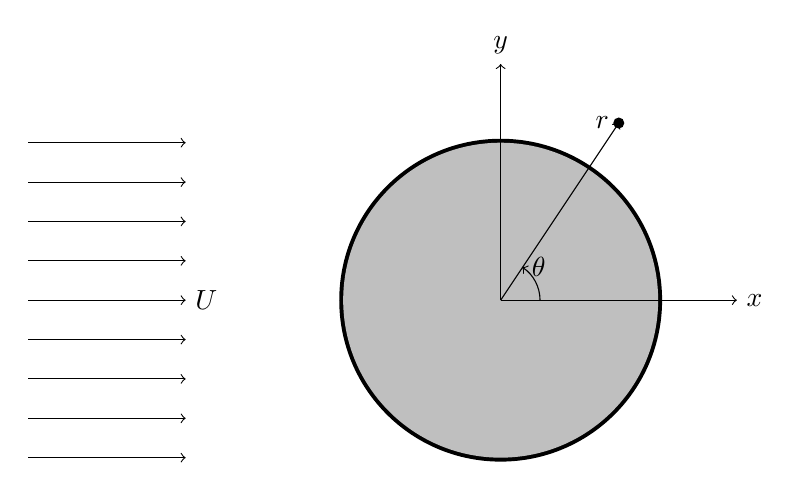
\begin{tikzpicture}
  \draw[->] (-6,0) -- (-4,0) node[right]{$U$};
  \draw[->] (-6,0.5) -- (-4,0.5) ;
  \draw[->] (-6,1) -- (-4,1) ;
  \draw[->] (-6,1.5) -- (-4,1.5) ;
  \draw[->] (-6,2) -- (-4,2);
  \draw[->] (-6,-0.5) -- (-4,-0.5) ;
  \draw[->] (-6,-1) -- (-4,-1) ;
  \draw[->] (-6,-1.5) -- (-4,-1.5) ;
  \draw[->] (-6,-2) -- (-4,-2);
  

   

    % Draw the circle
    \draw[line width =1mm] (0,0) circle(2); % Circle with radius 2
    \fill[gray!50] (0,0) circle(2); % Fill the circle with gray

    % Draw the line y = 2x
    \draw[->] (0,0) -- (1.5,2.25)  node[left]{$r$};
    \fill (1.5,2.25) circle (2pt);
     % Draw the axes
    \draw[->] (0,0) -- (3,0) node[right] {$x$};
    \draw[->] (0,0) -- (0,3) node[above] {$y$};
    \draw[->] (0.5,0) arc[start angle=0, end angle=57, radius=0.5] node[right]{$\theta$};

    % Mark the intersection points

\end{tikzpicture}


